\documentclass{article}
\usepackage{graphicx} % Required for inserting images

\usepackage{float}
\usepackage{dialogue}
\usepackage{tikz}
\usepackage{natbib}
\usepackage{setspace}
\usepackage{tabularx}

\usepackage{amsmath}
\usepackage{amsthm}
\usepackage{amssymb}
\usepackage{tcolorbox}

\DeclareMathOperator{\CostBlock}{CostBlock}
\newtheorem{theorem}{Theorem}
\newtheorem{proposition}[theorem]{Proposition}
\newtheorem{lemma}[theorem]{Lemma}
\newtheorem{definition}[theorem]{Definition}
\DeclareMathOperator{\minCost}{minCost}

\begin{document}
%\title{The Economics of Generative and Agentic AI}
\title{The Labor Economics of Agentic AI}
\author{John Horton\footnote{I used AI extensively to write this paper, particularly Claude 3.5 Sonnet and o1 pro from OpenAI. Thanks for complementing my labor, AI agents!}\\MIT \& NBER}
\date{\today{}}

\newcommand{\machine}[1]{\langle #1 \rangle}
\newcommand{\human}[1]{( #1 )}
\newcommand{\cost}[1]{C\{ #1 \}}
\newcommand{\costdo}[1]{C_H\{ #1 \}}
\newcommand{\costmanage}[1]{C_M\{ #1 \}}

\newcommand{\topic}[1]{\paragraph{#1}}
%\newcommand{\topic}[1]{#1}

\maketitle

\begin{abstract}
\noindent This paper presents a simple task-based model of Agentic AI and human labor.
The model focuses on the decision to use an AI for a task based on the cost of human prompting and evaluation versus the cost of human performance. 
Unlike other tasks models, it considers the interdependence of tasks in a sequence. 
Tasks can be efficiently ``chained'' together in the sense that each task produces someting that feeds into the next without human intervention.
A task might be added to an automated chain even if the human has an absolute advantage in that task in isolation, reversing the usual comparative advantage calculation.
\end{abstract}

\onehalfspacing
  
\section{Introduction}
The distinctive feature of generative AI is captured in its name: it generates---writing, code, images, music, and videos---in response to human requests, or ``prompts.''
Yet these model generations only become (potentially) economically valuable---counting as completed tasks---when humans judge these model outputs as suitable for their needs.
If the model outputs are generally poor or too unreliable, the human might eschew AI and do the task themselves.
This creates a practical question: what tasks be routed to an AI versus performed directly by a worker?
And if a job consists of multiple tasks, what should the allocation between human and machine be, collectively? 

Multiple AIs working in concert, or so-called ``Agentic AI,'' has captured the imagination of researchers and practitioners alike.
The enthusiasm reflects the essential correctness of the task-based view of production: many goods are produced by the completion of tasks.
Most tasks have a recursive sub-structure, allowing them to be decomposed into smaller, simpler tasks.
Those simpler tasks might more plausibly done by capable AIs rather than humans. 
But in designing such an AI, specialization in not just for humans.
The ``agentic'' of agentic AI captures the idea that an AI working on a particular task should be specialized for that task---it should have resources, knowledge and capabilities needed for that task and that task alone.
It is differentiated and specialized in the same way that a human worker might be specialized. 
While engineers might cast this as simply reflecting good software engineering principles---separation of concerns, modularity, clean interaces between sub-components---it also describes an effective organizational productive process.
In short, enthusiasm for Agentic AI is enthusiam for the division of labor---old wine in new bottles. 

The paper presents a simple task-based model of agentic AI and human labor.
As with other task-based models, the focus is on whether labor or capital (here, AI) is assigned the task.
In the model, the decision to use an AI is based on the cost of the human's ability to direct and evaluate the AI's output, compared to the human's ability to do the task directly.
This might seem like another way of stating that the task gets done by the factor of production with the comparative advantage in that task, but this is not the case:
the model considers the fact that each task is often an input to the next task in a sequence of tasks, and that the output of some previous task is the input to the focal task.
This consideration can profoundly change the allocation of tasks between humans and machines, even reversing the usual comparative advantage argument.

In the model, two or more tasks can be ``chained'' together and treated as a single task.
The machine is given responsibiity for the hand-off between tasks, with no human intervention between the completion of one task and the start of the next.
This chaining is potentially a source of enormous productivity gains, \emph{but} it requires powerful AI that can do each task with a high probability of success, as in the o-ring model of production \citep{kremer1993}.

This possibility of ``chaining'' automated tasks together can reverse comparative advantage calculations for individual tasks.
It can be efficient to use an AI for a task even if humans have a comparative advantage in that task, if chaining allows for a longer chain of tasks to be fully automated.
We can explore these considerations because we explicitly model the human costs of directing, or ``prompting,'' and judging AI outputs. 
This elaboration is also useful because it highlights where technological improvements are likely to occurr and what it means for AI to complement human capabilities.

Another advantage of considering the interdepdence of tasks is it allows us to consider the complementarity of AI improvements in their capabilities at different tasks.
First, for AI far away from automation, investments in AI capabilities offer no return because the AI is inframarginal.
Once above the threshold however and the human is replaced, improvements in AI capabilities ofter a return in that task alone. 
But once chained, improvements in AI capabilities at one task increases the return to investing in other tasks in the same chain.

This task but with chaining framework helps conceptuall reconcile competing views about automation in production. 
Some researchers emphasize task-level substitution between AI and labor \citep{autor2003skill, acemoglu2018automation}, while others argue that meaningful substitution happens primarily at the system level \citep{bresnahan2020artificial}. 
One could interpret the model as showing how task-level decisions aggregate into system-level automation through task chaining.

The model predicts that improvements in AI will inherently reduce labor use per unit of the good, and hence the price. 
But whether this increases or decreases the demand for labor even for that task depends on the elasticity of demand for that good in the product market.
As a historical touchpoint, consider that the enormous increases in agricultural were not manifested by humans eating 40x more food, but rather having a shrinking agricultural sector, in terms of headcount.
Perhaps even more important, the creation of new goods requiring new tasks is likely to be of first-order importance in the economy, and yet these are hard to model credibly---though it does seem likely that ``freed up'' labor will tend to create new goods that tend be complement that labor, not because of some technicalogical reason but simply because of the incentives to do so.
As such, the paper stays silent on these questions and does not offer a general equilibrium model of the economy.
The reason is simple: if AI has productivity effects that are so large they are worth paying attention to, the less likely we could say something meaningful in highly a stylized model.

\section{Economic treatment of technological innovation and labor markets}
% Good
One approach to understanding the impact of technology on labor markets has been to focus at the ``task'' level.
Goods are produced by the completion of tasks and those tasks can be assigned to the factor of production with the comparative advantage in that task.
This approach has been applied not just to technology but also to trade and offshoring.
But specifically with respect to AI and automation, the task-based view is that labor, by being more flexible \citep{acemoglu2011skills}, has an absolute advantage in ``new'' tasks, but that as time passes, they become susceptible to automation \citep{acemoglu2018}.

% Good
A contrasting view of technology is offered by \cite{bresnahan2020artificial}, who argues there has been no task-level substitution with the AI systems we actually see in production: ``the transition to ICT-based production has largely proceeded at the system level, not the task level.''
To the extent there is important labor-capital substitution, the argument is that it will happen at the system level.
There is a long tradition in studies of ICT to take a ``systems'' view---that ICT requires a reconfiguration of production to reap the benefits \citep{bresnahan2002information}. %(Cite Erik).

An argument for a task-based view with respect to generative AI is that it does tasks.
The things it can do well: analyzing data, writing reports, drafting communications, doing research, coming up with plans, etc., certainly seem like the kinds of tasks common across large numbers of workers.
Experimental evidence at knowledge worker tasks shows large productivity gains using ChatGPT for a collection of knowledge worker tasks \citep{noy2023experimental}.
The fraction of tasks currently performed by workers in the US that might be done or augmented with LLMs is considerable \citep{eloundou2023gpts}.
This is perhaps not surprising given the models were explicit trained on data that was generated by humans doing these tasks.
This stands in contrast to, say, ICT like databases, servers, data centers, recommender systems, etc. are better characterized as technologies that can be used to build systems that might do some tasks or replace whole collections of tasks.  
The product market success and adoption of ChatGPT is a testament to this: there are 100M users of OpenAI and presumably, many are using it for their work.
Even the names of these technologies indicate their role of helping individuals: the names people use like ``co-pilot'' and ``assistant'' 

The literature to date on AI specifically (as opposed to automation more generally) in the task-based tradition has emphasized AI as a prediction technology \citep{agrawal2019}.
While forecasting and prediction are certainly key firm tasks, relatively few workers have that as a task \emph{per se}. 
By comparison, the outputs of generative AI---things like writing, research, or analysis (which could include prediction) are commonplace. 
As a case in point, on ONET, only 22 occupations are returned for the search term ``predicting.'' 
By comparison, the occupations returned for ``communicating,'' ``writing'' and ``analysis'' are 426, 332, and 408, respectively. 
Furthremore, it really does make sense to think of tasks as having outputs that feed into other tasks.

\section{A model of production}

We begin by analyzing the production process for a single task before extending to multiple interdependent tasks.
This approach allows us to isolate the fundamental economic trade-offs before introducing task interdependencies.

Consider a worker completing some sequence of tasks as part of their job.
If they choose to use an AI, the human asks the AI to perform the task with a ``prompt''---a request to the model. 
The AI tries to perform the task, generating output.
The worker then evaluates the output to decide if it is suitable for their needs. 
If it is, the worker can continue to the next task; 
if it is not, the worker can try to modify the prompt and re-evaluate the new output until the need is satisfied. 
Figure~\ref{fig:flow} shows this process.

\begin{figure}
  \caption{Using AI at Work} \label{fig:flow}
  \includegraphics[width = \textwidth]{images/flow.png}
\end{figure}

To make predictions, we need to make some assumptions about the costs of the different components of the process.
Let us define the following:
\begin{itemize}
    \item $c_h$: The cost of human performance of the task
    \item $c_p$: The cost of providing instructions (``prompting'') to the AI
    \item $c_e$: The cost of evaluating the AI's output
    \item $q$: The probability that the AI successfully completes the task, given the prompt
\end{itemize}

Let $c_m = c_p + c_e$ denote the total ``management'' costs associated with using the AI.
In terms of notation, the tasks are numbered 1, 2, 3, and so on.
When a human performs the task, we denote this as $\human{\cdot}$ with cost $\cost{\human{\cdot}} = c_h$.
When an AI attempts the task under human supervision, we denote this as $\machine{\cdot}$.

If the AI fails (with probability $1-q$), the human can provide a new prompt and evaluate a new attempt, incurring costs $c_m$ again.
Attempts are independent, leading to the following result:

\begin{lemma}[Single Task Automation Criterion] \label{lemma:single}
A task should be automated if and only if $\cost{\machine{1}} < \cost{\human{1}}$, which occurs when $c_m/q < c_h$.
\end{lemma}
\begin{proof}
The expected cost of using the AI is:
\begin{align*}
    \cost{\machine{1}} &= c_m \sum_{k=1}^{\infty} k q(1-q)^{k-1} \\
    &= c_m/q
\end{align*}
where the second line follows from the standard result for the expectation of a geometric distribution.
Therefore, automation is optimal when $c_m/q < c_h$.
\end{proof}

This criterion has intuitive comparative statics.
Automation becomes more attractive when:
\begin{enumerate}
    \item Human performance costs ($c_h$) are high
    \item Management costs ($c_m$) are low
    \item AI success probability ($q$) is high
\end{enumerate}

Note that improvements in tools for prompting and evaluation can reduce management costs and thus make automation more attractive, even if the AI's success probability is unchanged.

\begin{tcolorbox}
\subsection{Discussion: Is that what prompting is really like?}
There is some unrealism in the model that makes the presentation simpler but elides from pracical considerations.
First, the model assumes that failures and sucesses are independent, when they might be correlated.
A bad initial prompt might lead to a bad output, which might be hard to fix, causing the system to get stuck and perhaps never succeed. 
Second, we might expect that subsequent attempts are easier fix and less costly, perhaps requiring less work. 
While true, the main economic feature to capture is that a low $q$ raises management costs.
The simplicity of the math makes it easier to see the main points and the model is not intended to be a literal description of the process.
\end{tcolorbox}

\begin{tcolorbox}
\subsection{Discussion: Are management costs low?}
Prompting and evaluation are human skills.
How high are $c_p$ and $c_e$?
One question is simply how long theose tasks take to do; other is how widely held these skills are in the population.
There is no inherent reason to think that eitehr will itself be a low-skill task.
Most of management is deciding what you want done, asking right people to do it, in a way that leads to an effective outcome, and then monitoring the process to see if it acheiving the desired goals.
\end{tcolorbox}

\begin{tcolorbox}
\subsection{Comment: Managing an AI is similar to managing people}
The decision to use an AI bears similarities to the decision to delegate some task to a subordinate or team.
Doing this well requires being a judge of talent, scoping and explaining projects in ways people will understand, giving good, actionable feedback, and so on. 
And conditional upon delegation, the skill of using AI bears similarities to the management of people and teams. 
Deciding whether the output is sufficient requires judgment, whether the output is human-produced or otherwise. 
But given humans are harder to change the machines, it seems likely that AIs will continue to be modified to make it so that humans can manage them more easily. 
\end{tcolorbox}

\begin{tcolorbox}
\subsection{Discussion: Is the output a search good, inspection good, or credence good?}
The costs of judging the model's output could vary widely depending on the nature of the task and the person assiged to it.
An analogy can be drawn to the process by which consumers evaluate goods. 
Search goods are trivially easy to evaluate, whereas inspection goods might have prohibitively expensive evaluation costs. 
Or, goods that are credence goods---goods that that the consumer has to take on faith work---might have de facto infinite evaluation costs.
Some goods might be inspection goods for some people and search goods for others. 
If a task requires true expertise to evaluate, the cost of evaluation might be de facto infinite.
\end{tcolorbox}

\begin{tcolorbox}
\subsection{Comment: There will be efforts to lower evaluation costs}
Economics classifies goods by the evaluation costs required to assess them, with some tasks like LLM-generated ad copy requiring minimal oversight while others like surgical plans or judicial opinions demand much more rigorous evaluation.
For some tasks, the human is the final arbiter and can immediately decide if the outcome is sufficient, with no further sources needed. 
For example, a model-generated meeting agenda can be evaluated at a glance. 
Other information goods require more costly inspection, like computer code which LLMs can produce but must be tested across different inputs (though test-driven development helps systematize this verification). 
Similarly, math problems often use guess-and-verify approaches or require checking if answers are sensible, even when following standard procedures. 
While critics often point to ChatGPT's factual errors, AIs that can cite sources effectively transform these inspection goods into more easily verifiable search goods.
\end{tcolorbox}

\begin{tcolorbox}
\subsection{Comment: One-off nature of AI output hampers the ability to use reviews to evaluate}
  Some information goods are consumed over time, and learning about their quality might take time. 
A person might not know if they enjoyed a movie until they have actually watched it. 
For information experience goods, we tend to rely heavily on reviews. 
But this only works when many people potentially evaluate the same good. 
With generative AI, the information good is likely generated uniquely for that particular worker. 
A non-lawyer could not verify whether a commercial contract is likely to hold up to scrutiny by the courts. 
A course of advised medical treatment might be very difficult to judge by a non-expert.
\end{tcolorbox}

\begin{tcolorbox}
\subsection{Discussion: Model evaluation in a work context is an economic consideration, not a purely technical one}
Consider the task ``answer questions about the text in a document'' and whether an AI can do this task depends on the payoff to doing it correctly. 
The firm might be fine letting a machine do low-level customer service support; we might be very hesitant to let it handle queries from major institutional investors, in part because what constitutes ``good enough'' differs.
But also, the next task might be follow-questions about the state of the business that only the CFO can credibly answer.
\end{tcolorbox}

\subsection{Two task production with chaining}
Now we move from a single task to two tasks in sequence. 
While we will consider arbitrary sequences of tasks, most of the important points can be illustrated with just two tasks.
Consider a job consisting of two sequential tasks with AI success probabilities $q_1$ and $q_2$.
With two tasks, there are four possible production arrangements:
\begin{align*}
    \cost{\human{1}\human{2}} &= 2c_h & \text{(fully human)} \\
    \cost{\machine{1}\machine{2}} &= \frac{c_m}{q_1} + \frac{c_m}{q_2} & \text{(independent automation)} \\
    \cost{\machine{1}\human{2}} &= \frac{c_m}{q_1} + c_h & \text{(partial automation)} \\
    \cost{\human{1}\machine{2}} &= c_h + \frac{c_m}{q_2} & \text{(partial automation)} \\
\end{align*}
However, there is a fifth arrangement where the completed first task is used as input for the second task without human intervention.
When tasks are chained, denoted by $\machine{1|2}$, they are executed sequentially by the AI with a single prompt and final evaluation.
\begin{align}
\cost{\machine{1|2}} &= \frac{c_m}{q_1q_2} & \text{(chained automation)}
\end{align}

\begin{figure}
  \caption{Cost minimization with two tasks} \label{fig:two_tasks}
  \includegraphics[width = 0.8 \textwidth]{images/two_tasks.pdf}
\end{figure}

A key implication is that chaining can be optimal even when humans have a comparative advantage in one of the tasks in isolation, as formalized in the following lemma:

\begin{lemma}[Task Interdependence] \label{lemma:interdependence}
A task might be optimally automated as part of a chain even when humans have a comparative advantage in that task in isolation.
Specifically, $\cost{\human{1}\machine{2}} < \cost{\machine{1}\machine{2}}$ does not imply $\cost{\human{1}\machine{2}} < \cost{\machine{1|2}}$.
\end{lemma}

\begin{proof}
Consider $q_1 = 3/5$, $q_2 = 4/5$, $c_m = 1$, and $c_h = 3/2$.
For task 1 in isolation, human performance is cheaper: $c_h = 3/2 < 5/3 = c_m/q_1$.
However:
\begin{align*}
    \cost{\human{1}\machine{2}} &= c_h + \frac{c_m}{q_2} = \frac{3}{2} + \frac{5}{4} = \frac{11}{4} \\
    \cost{\machine{1|2}} &= \frac{c_m}{q_1q_2} = \frac{25}{12} < \frac{11}{4}
\end{align*}
Thus, chaining is optimal despite human comparative advantage in task 1.
\end{proof}

For the more general case, fix $n$ tasks with success probability $q \in (0,1)$ and costs $c_m = 1$, $c_{h,i} = c_h$ for all $i$.
We require:
\begin{align*}
c_h &< \frac{1}{q} && \text{(human cheaper per task)} \\
n c_h &> \frac{1}{q^n} && \text{(machine chain cheaper overall)}
\end{align*}
These conditions are compatible when:
\[
\frac{1}{n q^n} < c_h < \frac{1}{q}
\]
which requires $q^{n-1} < n$.
We can pick any $c_h$ in the open interval $(\frac{1}/{nq^n}, \frac{1}{2})$ to satisfy the conditions.

A direct implication of the above is that improvements in the AI capabilities of an adjacent task can cause a a task to go directly from being done by human to being done by machine (as part of a chain).
Assume the following baseline parameters:
\begin{align*}
    c_h &= 1, \\
    c_m &= 1, \\
    q_1 &= 0.6, \\
    q_2 &= 0.8.
\end{align*}
The cheapest option is fully human production:\
\begin{align*}
    \cost{\human{1}\human{2}} = 2.
\end{align*}
Thus, both tasks are done by humans. In particular, \textbf{Task 1 is performed by a human.}
Now suppose we invest in improving the AI's success probability for Task 2, raising $q_2$ from $0.8$ to $1.0$. The new costs are:
\begin{enumerate}
    \item \textbf{Human-Human:}
    \begin{align*}
        \cost{\human{1}\human{2}} &= 2 \quad \text{(unchanged)}.
    \end{align*}
    \item \textbf{Chaining:}
    \begin{align*}
        \cost{\machine{1|2}} &= \frac{c_m}{q_1 q_2} \\
        &= \frac{1}{0.6 \times 1.0} = \frac{1}{0.6} = 1.666\ldots
    \end{align*}
\end{enumerate}
With $q_2 = 1.0$, the cheapest option is now chaining:\
\begin{align*}
    \cost{\machine{1|2}} = 1.666\ldots < \cost{\human{1}\human{2}} = 2.
\end{align*}
Although Task 1's parameters ($c_h, q_1$) are unchanged, it flips from human to machine because chaining amortizes the management cost $c_m$ across both tasks. 
The improvement in Task 2's success probability reduces the expected cost of chaining both tasks, making automation optimal.
This example illustrates how investments in one task's AI performance can cause an adjacent task to switch to automation, even when the adjacent task itself has not improved. 
The interdependence of tasks through chaining creates complementarities in automation decisions.
This effect can be seen graphically in Figure~\ref{fig:two_tasks}.
Note that that the $\human{1}\human{2}$ to $\machine{1|2}$ frontier is sloped, meaning an increase in $q_2$ can bring you directly from human to automation (in a chain) but not to automation in isolation.

\begin{tcolorbox}
  \subsection{Comment: The division of labor tends to create interdependence of tasks within jobs}
  Economic forces create dependencies between tasks within jobs. 
  Consider pin manufacturing: each step (washing wire, spooling, straightening, cutting, grinding) serves as input to the next, with failures at any point endangering the final product. 
  The limit to this division of labor is not technical but economic, as Smith noted.
  These tasks could be split more finely, but the costs of switching and communication between workers would outweigh the benefits.
  While specialization is primarily constrained by market size, it also faces switching and communication costs when work is handed off between workers. 
  These costs create serial dependencies between tasks done with a job---the tasks that make up a job are precisely those tasks that are hard to hand-off to someone else. 
  It is unclear why this would be different when we try to automate tasks with machines.
  % endregion: Division of labor creates interdependence of tasks within jobs
\end{tcolorbox}

The optimal assignment of tasks to humans or AI depends not just on isolated comparative advantage, but on the relationships between tasks.

\begin{tcolorbox}
\subsection{Comment: Chained tasks create systems}
Once a task is changed, it can be thought of as a new, single task.
What constitutes a ``task'' moves to higher and higher levels of abstraction: 
From ``find typos in this ad copy'' to ``create ad copy'' to ``create a marketing campaign, launch, execute and monitor performance'' to ``increase sales'' to ``run the business profitably'' to $\ldots$.  
Note that with this chaining tasks can become increasingly large and abstract as models increase, generating something that looks like an entire system and not just a task \cite{bresnahan2020artificial}.
\end{tcolorbox}

\begin{tcolorbox}
\subsection{Comment: Chained tasks can be re-factored by machines as they see fit}
We might also imagine that once fully chained, the system is free to ``re-factor'' production within the chain---it simply takes inputs and generates outputs.
The details of how this is done is up to the model. 
In the language of our model, system-level substitution would just be characterized as long chains of task automation.
\end{tcolorbox}

\subsection{Properties of Chained Production}
The cost gradient with respect to AI capabilities has different properties under chaining versus independent automation.
For independent automation, improving $q_i$ only affects tasks where the AI is used in isolation.
Under chaining, we have:

\begin{proposition}[Chain Complementarity]
In chained production, improvements in AI capabilities for different tasks are substitutes in cost reduction:
\begin{equation}
    \frac{\partial^2}{\partial q_1 \partial q_2} \cost{\machine{1|2}} = \frac{c_m}{q_1^2q_2^2} > 0
\end{equation}
\end{proposition}

This creates incentives for balanced investment in AI capabilities across chain components, as improvements in the weakest link generate the largest cost reductions.

\subsection{Effect of AI Improvements}
The impact of improving AI capabilities (increasing $q_1$ or $q_2$) varies systematically across production arrangements:

\begin{proposition}[Comparative Statics]
The effect of improving AI capabilities has the following properties:
\begin{enumerate}
\item In human-only production, improvements in AI have no effect on costs:
\[\frac{\partial \cost{\human{1}\human{2}}}{\partial q_i} = 0 \text{ for } i \in \{1,2\}\]
\item In independent AI production, improvements reduce costs independently:
\[\frac{\partial \cost{\machine{1}\machine{2}}}{\partial q_i} = -\frac{c_m}{q_i^2}, \quad \frac{\partial^2 \cost{\machine{1}\machine{2}}}{\partial q_1 \partial q_2} = 0\]
\item In mixed production, only improvements in the automated task matter:
\[\frac{\partial \cost{\machine{1}\human{2}}}{\partial q_1} = -\frac{c_m}{q_1^2}, \quad \frac{\partial \cost{\machine{1}\human{2}}}{\partial q_2} = 0\]
\item In chained production, improvements are complementary:
\[\frac{\partial \cost{\machine{1|2}}}{\partial q_i} = -\frac{c_m}{q_i^2q_j}, \quad \frac{\partial^2 \cost{\machine{1|2}}}{\partial q_1 \partial q_2} = \frac{c_m}{q_1^2q_2^2} > 0\]
where $j \neq i$.
\end{enumerate}
\end{proposition}

We now characterize when tasks should be chained together versus performed independently.
The analysis reveals that the optimal structure depends on both the absolute and relative success probabilities of the component tasks.
We begin with the fundamental decision of whether to chain two automated tasks:

\begin{proposition}[Optimal Chaining for \(n\) Tasks]
  Chaining \(n\) automated tasks is optimal if and only if:
  \[
  \sum_{i=1}^n \prod_{j \neq i} q_j > 1.
  \]
  \end{proposition}
  
  \begin{proof}
  Chaining is optimal if:
  \[
  \frac{c_m}{\prod_{i=1}^n q_i} < \sum_{i=1}^n \frac{c_m}{q_i}.
  \]
  Dividing by \(c_m > 0\) and multiplying by \(\prod_{i=1}^n q_i\) yields:
  \[
  1 < \sum_{i=1}^n \prod_{j \neq i} q_j.
  \]
  Thus, chaining is optimal if and only if the inequality holds.
  \end{proof}

For a more constructive example with $n$ tasks, 

This result has an intuitive interpretation: chaining eliminates duplicate management costs but increases the chance of overall failure.
The sum of success probabilities must exceed one to make this trade-off worthwhile.
The basic chaining criterion extends to longer sequences in systematic ways:

\begin{proposition}[Chain Composition]
Optimal task chains have the following properties:
\begin{enumerate}
\item A cost-minimizing sequence cannot contain a chain where the success probabilities sum to less than one
\item When choosing which tasks to chain together, higher probability tasks should be chained first
\end{enumerate}
\end{proposition}

\begin{proof}
For part (1), consider any three consecutive tasks in a chain with probabilities $(q_l, q_\epsilon, q_r)$.
If $q_l + q_\epsilon + q_r < 1$, then:
\[\frac{1}{q_lq_\epsilon q_r} > \frac{1}{q_l} + \frac{1}{q_\epsilon} + \frac{1}{q_r}\]
Therefore breaking the chain would reduce costs.

For part (2), consider combining task $q$ with either $q_H$ or $q_L$ where $q_H > q_L$.
Chaining with $q_H$ is preferred when:
\[q(q_H - q_L) < q_H - q_L\]
which always holds when $q_H > q_L$ and $q < 1$.
\end{proof}

For the the $n$ task case, consider a sequence of \(n\) tasks, each of which can be:
\begin{enumerate}
    \item Done by humans, with cost \(c_{h,i}\), assumed success probability \(1\),
    \item Done by the machine:
    \begin{itemize}
        \item \textbf{Independently}: The expected cost is \(\frac{c_m}{q_i}\),
        \item \textbf{Chained}: For a block of tasks \(B \subseteq \{1, \dots, n\}\), the cost is \(\frac{c_m}{\prod_{i \in B} q_i}\).
    \end{itemize}
\end{enumerate}

The \textbf{optimal cost} \(C(q_1, \dots, q_n)\) is determined by solving:
\[
C(q_1, \dots, q_n) = \min_{\substack{\text{a partition of } \{1, \dots, n\} \\ \text{into blocks } B_1, \dots, B_k}} \sum_{\alpha=1}^k \CostBlock(B_\alpha),
\]
where each block \(B_\alpha\) is either:
\begin{itemize}
    \item A \textbf{human block}: \(\sum_{i \in B_\alpha} c_{h,i}\),
    \item A \textbf{machine chain block}: \(\frac{c_m}{\prod_{i \in B_\alpha} q_i}\).
\end{itemize}

This minimization is often solved using a DP, building \(C(q_1, \dots, q_n)\) from smaller subproblems.
The cost function \(C(q_1, \dots, q_n)\) is defined as the \textbf{minimum} over all partitions \(P\). For a given partition \(P = \{B_1, \dots, B_k\}\), the cost is:
\[
C_P(q_1, \dots, q_n) = \sum_{\alpha=1}^k
\begin{cases}
\sum_{i \in B_\alpha} c_{h,i}, & \text{if } B_\alpha \text{ is a human block}, \\[6pt]
\frac{c_m}{\prod_{i \in B_\alpha} q_i}, & \text{if } B_\alpha \text{ is a machine chain block}.
\end{cases}
\]

The optimal cost is:
\[
C(q_1, \dots, q_n) = \min_{P} C_P(q_1, \dots, q_n).
\]

This implies that \(C(q_1, \dots, q_n)\) is a \textbf{piecewise minimum} of sums of terms involving \(\frac{1}{q_i}\). Consequently:
\begin{itemize}
    \item \(C(q_1, \dots, q_n)\) is continuous but generally only \textbf{piecewise differentiable}.
    \item At points where the optimal partition changes, \(C(q_1, \dots, q_n)\) may have “kinks” or non-smooth transitions.
\end{itemize}

For any region where a single partition \(P\) is optimal, the partial derivatives of \(C(q_1, \dots, q_n)\) match those of \(C_P(q_1, \dots, q_n)\). Using the envelope theorem:
\begin{itemize}
    \item \(\frac{\partial C}{\partial q_i} \leq 0\), with equality if task \(i\) is handled by humans (since \(q_i\) does not affect human costs).
    \item If tasks \(i\) and \(j\) are in the \textbf{same machine chain block}, then:
    \[
    \frac{\partial^2 C}{\partial q_i \partial q_j} > 0,
    \]
    reflecting \textbf{complementarity}. Otherwise, the cross partials are zero.
\end{itemize}

\begin{enumerate}
    \item \textbf{Human-assigned tasks}: If task \(i\) is assigned to humans, then:
    \[
    \frac{\partial C}{\partial q_i} = 0.
    \]

    \item \textbf{Stand-alone machine tasks}: If task \(i\) is handled independently by the machine, then:
    \[
    \frac{\partial C}{\partial q_i} = -\frac{c_m}{q_i^2}, \quad \frac{\partial^2 C}{\partial q_i \partial q_j} = 0 \text{ for } j \neq i.
    \]

    \item \textbf{Chained machine tasks}: If tasks \(i\) and \(j\) are in the same machine chain block, then:
    \[
    \frac{\partial C}{\partial q_i} = -\frac{c_m}{q_i^2} \cdot \frac{1}{\prod_{k \neq i} q_k},
    \]
    \[
    \frac{\partial^2 C}{\partial q_i \partial q_j} = \frac{c_m}{q_i^2 q_j^2} \cdot \frac{1}{\prod_{k \not\in \{i, j\}} q_k} > 0.
    \]
    Tasks in the same chain exhibit \textbf{complementarity}, but tasks in different chains or assigned to humans do not (\(\frac{\partial^2 C}{\partial q_i \partial q_j} = 0\)).
\end{enumerate}

\begin{enumerate}
    \item \textbf{Monotonicity}: Increasing any machine success probability \(q_i\) (\(q_i \uparrow\)) never increases the optimal cost:
    \[
    \frac{\partial C}{\partial q_i} \leq 0.
    \]
    This inequality is strict if task \(i\) is in a machine block.

    \item \textbf{Complementarity}: Tasks within the same chain exhibit complementarity:
    \[
    \frac{\partial^2 C}{\partial q_i \partial q_j} > 0 \quad \text{if tasks } i \text{ and } j \text{ are in the same chain block}.
    \]
    Tasks in different blocks or assigned to humans have zero cross partials.

    \item \textbf{Piecewise Differentiability}: Across regions where the optimal partition changes, \(C(q_1, \dots, q_n)\) may exhibit kinks but remains continuous and everywhere bounded.
\end{enumerate}

The comparative statics of the 2-task case extend naturally to \(n\)-task settings:
\begin{itemize}
    \item Human tasks remain unaffected by \(q_i\).
    \item Stand-alone machine tasks have monotonic but independent cost reductions.
    \item Chained machine tasks exhibit complementarity among tasks in the same chain.
\end{itemize}

\begin{tcolorbox}
  \subsection{Model innovation will focus on tasks that are inputs and outputs of each other}
  Because of chaining, it matters what tasks are ``next'' to each other in some productive process, because tasks that have a high ability to be automated can be chained together.
  In different occupations, different tasks might appear adjacent to each other. 
  Writing might appear next to hundreds of different tasks, from ``send your economics paper to a journal (after writing)'' to ``drop your maintence report slip into a box'' at the end of a shift driving a bus.
  As such, we can get ``automation dispersion'' where tasks are automated in some production settings but not others because of task adjacency.
  \end{tcolorbox}
  
The \(n\)-task generalization preserves the key qualitative insights: improvements in AI capabilities lower costs and create synergies when tasks are chained.

\subsection{Longer tasks sequences}
Now we will consider a job that is a sequence of tasks to be performed $1, 2, \ldots n$.
Note that with an $n$ task jobs, there are $2^{n-1}$ possible task partitions.
And each singleton can be done by a human or a machine; each sequence is done only by a machine.

The cost minimization problem is equilvalent to finding the shortest path in a tree.
To grow the tree, start with the first task.
It can be automated or done by a human.
It then has up to two children---the next task is either machine or human, and if machine, it could also be part of a chain.
Figure~\ref{fig:tree} illustrates the tree. 
The tree grows to, worse-case, $2^n$ children where $n$ is the number of tasks.
It would be less than this because human-done nodes only have one child: either machine or human.

\begin{figure}
\caption{The possible production scenarios with an $n=2$ task job}
\label{fig:tree}
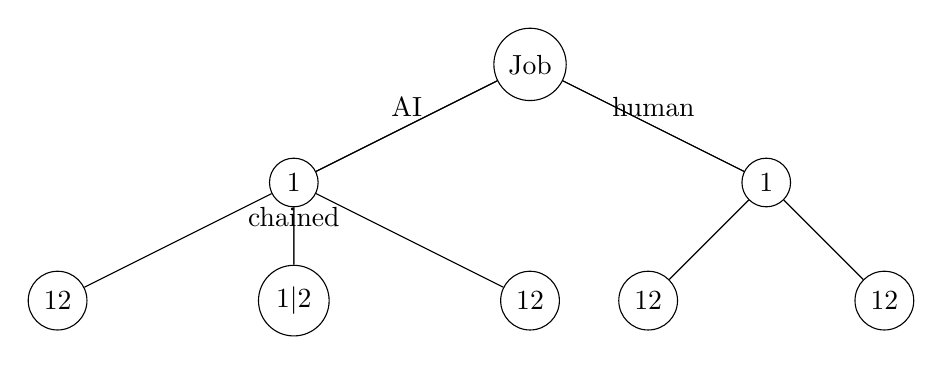
\begin{tikzpicture}[
  level/.style={sibling distance=60mm/#1}
]
\node[circle, draw] (S) at (0,0) {Job}
  child {node[circle, draw] (A) {$\machine{1}$}
    child {node[circle, draw] (AA) {$\machine{1}\machine{2}$}}
    child {node[circle, draw] (AAC) {$\machine{1|2}$}} 
    child {node[circle, draw] (AH) {$\machine{1}\human{2}$}} 
  }
  child {node[circle, draw] (H) {$\human{1}$}
    child {node[circle, draw] (HA) {$\human{1}\machine{2}$}}
    child {node[circle, draw] (HH) {$\human{1}\human{2}$}}
  };
\path (S) edge node[midway, above] {AI} (A);
\path (S) edge node[midway, above] {human} (H);
\path (A) edge node[midway, above] {chained} (AAC);
\end{tikzpicture}
\end{figure}

Finding the minimum cost chain is a dynamic programing problem.
Consider a sequence of $n$ tasks that must be completed sequentially. 
Each task $i \in \{0,\ldots,n-1\}$ can be completed either by a human at cost $c_h[i] \in \mathbb{R}_+$ or attempted by an AI with success probability $q[i] \in (0,1]$.
Multiple consecutive tasks can be assigned to the AI as a single chain, incurring a fixed management cost $c_m \in \mathbb{R}_+$ per chain. 
When tasks $i$ through $j$ are chained, the expected cost is $\frac{c_m}{\prod_{k=i}^j q[k]}$, reflecting the expected number of attempts needed for success.

\begin{definition}[Minimum Completion Cost]
Let $V(i)$ denote the minimum expected cost to complete tasks $i$ through $n-1$. Then:

\begin{equation}
V(i) = \min\left\{
\begin{array}{l}
c_h[i] + V(i+1), \\[1ex]
\displaystyle\min_{j \geq i} \left\{\frac{c_m}{\prod_{k=i}^j q[k]} + V(j+1)\right\}
\end{array}
\right\}
\end{equation}

with boundary condition $V(n) = 0$.
\end{definition}

\begin{theorem}[Optimal Policy]
The optimal assignment can be found by solving the dynamic program above in $O(n^2)$ time. At each state $i$, the optimal action is either:
\begin{enumerate}
    \item Assign task $i$ to human (cost $c_h[i]$), or
    \item Chain tasks $i$ through $j^*$ to AI, where:
    \begin{equation}
        j^*(i) = \arg\min_{j \geq i} \left\{\frac{c_m}{\prod_{k=i}^j q[k]} + V(j+1)\right\}
    \end{equation}
\end{enumerate}
The minimum total cost is given by $V(0)$.
\end{theorem}

\begin{proof}
The optimality follows from standard dynamic programming arguments. The boundary condition ensures well-definedness, and the principle of optimality holds as the problem exhibits optimal substructure: the optimal solution to subproblem $i$ through $n-1$ depends only on optimal solutions to subproblems $j+1$ through $n-1$ for $j \geq i$. The computational complexity follows from the fact that for each state $i$, we must evaluate at most $n-i$ possible chain lengths.
\end{proof}
  
What would determine the use of AI? 
Clearly the capabilities of the model itself---if the model will fail with a high probability, using it is less attractive.
Tasks that are expensive for humans to do are natural candidates for automation.

% region: Chaining tasks 

% endregion: Chaining tasksh

% region: Division of labor creates interdependence of tasks within jobs

\begin{tcolorbox}
\subsection{Comment: Ability implies judgement but lack of ability does not imply lack of judgement}
Do not deny the antecedent.
While the ability to perform a task often implies the ability to evaluate it (as performers must understand their goal), the reverse is not necessarily true---there are many cases where humans can effectively judge and direct task completion without being able to execute the task themselves. 
This is particularly relevant for highly skilled work, where the pool of qualified evaluators may be larger than those who can perform the task, and mirrors traditional management relationships where managers direct work they cannot personally execute. 
Just as a person with broken arms could still evaluate if a coffee was properly served despite being unable to serve it themselves, the key insight is that prompting and judgment capabilities can be decoupled from task execution abilities when delegating work to AI systems.
\end{tcolorbox}


\begin{tcolorbox}
\subsection{Comment: AI systems could potentially evaluate their own outputs}
While AI systems could potentially evaluate their own outputs, this misses a key point: if an AI model could reliably improve its own evaluation process, those improvements likely would already be incorporated into the model's training and deployment.
Modern AI systems do engage in more sophisticated self-evaluation and reasoning during inference. 
However, what remains is human asking and human evaluation.
This could be entirey deskilled, reduced to cliking a button and rubber-stamp acceptence of what comes out of the model---similar to using a vending machine.
But is could also remain a highly skilled task on both ends.
\end{tcolorbox}

% \subsection{Innovation in complementary human skills}
% We are likely to see investment not only in direct model capabilities, but the ways in which they can be prompted and the results evaluated. 
% Citations, RAG, eliminate hallucinations are all manifestatons of this. 

\subsection{Incentives for investment}
One concern in Acemoglu model is what he calls ``so-so'' technologies that automate but show little net productivity benefit, merely displacing labor: ```Examples of so-so technologies include automated customer service, which has displaced human service representatives but is generally deemed to be low quality and thus unlikely to have generated large productivity gains.''
How likely is it that a ``so-so'' technology will emerge?
If we think of technological improvements as being endogenous, not that it only makes sense to invest in some AI technology if the firm can overshoot the break-even condition. 
Recall that the firm is indifferent to using AI when $c_m / \bar{q} = c_h$. 
Let us suppose the current state of the art is such that $q_0 < \bar{q}$.
Small improvements from $q_0$ provide no value until they exceed $\bar{q}$. 
If the firm can get the AI technology up to $q^*$, and let us suppose you will sell $x$ units at the ``old'' price, 
the firm's cost-savings will $(c_h - c_m / q^*) x = C_{q_0}(q^*)$, where $C$ is the one-time cost of improving the technology.

The optimal investment is thus $q^* = \sqrt{\frac{x}{|C'(q^*)|}}$.
It will only be made, however, if profitable to do so, considering the full costs of $C_{q_0}(q^*)$.
In short, if the R\&D gets done, it's likely only to be done of its important (large $x$) and if it is done, it is likely to overshoot the status quo considerably.  
It also seems likely, given that nature of AI, that once it is deployed, usage provides training data that enables continuous improvement in $q$, furthering lowering costs. 
Human workers also learn, but that human capital is not easily transferred to other workers. 

% A feature of modern ML research is how little of it has been direct, secretive R\&D to gain competitive advantage, and done more like basic research. 
%This makes sense if most of these technologies were far from commercialization.
% Let us suppose the current state of the art is such that $q_0 < \bar{q}$.
% Small improvements from $q_0$ provide no value until they exceed $\bar{q}$. 
% For quality level $q^*$ with market size $x$, the cost savings are $\left(c_h - \frac{c_m}{q^*}\right)x$
% Let $C_{q_0}(q^*)$ be the one-time cost of improving technology from $q_0$ to $q^*$. The optimal investment level satisfies:
% \begin{equation}
%     q^* = \sqrt{\frac{x}{|C'(q^*)|}}
% \end{equation}
% We observe more significant technological advances in domains with larger potential markets, if success is possible.
% The shape of $C_{q_0}(q^*)$ is crucial in determining investment patterns. 
% Steeper cost functions reduce optimal investment levels, even in the presence of large markets.
% The self-driving car industry provides an instructive example of these dynamics.
% Safe autonomous driving requires extremely high reliability---$\bar{q} \approx 0.9999$.
% The potentia market is enormous, creating a very large $x$ in our framework.


% \subsection{Labor-labor substition}
% Even if only some tasks are automated, it still might facilitate labor-labor substitution.
% This might change who eligible to fulfill some role in the productive process.
% To the extent there is some different in the requirements to do some task, ask for some task to be done, and evaluating the output of that ask, there is a possibility to use different kinds of workers in a productive task.

% In light of the change in what is delegated, I discuss how labor-labor substitution might change who performs a task. 
% In particular, job redesign will take advantage of the fact that skills in judging output are separate from the skill of creating some output.
% There are food critics who cannot cook; record producers who cannot play instruments; technologists who cannot program, and so on.
% As AI makes it so that humans no longer have to do every task in a job, AI might open up jobs to people who are otherwise blocked by a skill they lack.

% There are likely to be numerous tasks when prompting and judgment can lead to good outcomes even when the human offering those judgments cannot do it themselves.
% One reason is that the pool of people who can offer judgment is larger than the pool that can do the task. 
% This might be particularly true for tasks that require a great deal of skill.

\subsection{What it means for an occupation to ``disappear''}
Although there are advantages to thinking in terms of tasks, most labor market participants thing in terms of ``occupations.'' 
Our training and human capital acquistion is structured as occupations.
People want to know which whole occupations will disappear, and what occupations have good prospects. 

\begin{tcolorbox}
\subsection{Comment: Disappeared occupations often just gave prompting and judging tasks to customers}
The approach gives a way to think about an occupation ``disappearing.''
In the model, an occupation only disappears when all of its task are subsumed in an automation chain.
In this case, AI, but we can think of AI as capital more generally that can be directed by humans. 

Take an job that truly disappeared: elevator operator. 
The tasks were 1) ``Announce the direction of the elevator,'' 2) ``ask people what floors they are going to'' 3) ``bring the elevator to the appropriate floors'', 4) ``open the doors'' as well as some other non-sequential tasks like inspect for defects or machine failures.  
This got turned into an automation chain where the customer was given the ``prompting'' task of selecting a floor; the evaluation task is just seeing that the elevator was the appropriate floor---an inspection good.
If it was hard to know if you had gotten the right floor, we might expect that task to still be done by humans.

Or consider retail in the past where all items were on shelves behind counters. 
The consumer would prompt the clerk to fetch items (perhaps asking for recommendations) and then the clerk would handle the merchandize. 
It was not until Piggly Wiggly allowed customers to select the merchandise directly that this task disappeared. 
\end{tcolorbox}

\begin{tcolorbox}
\subsection{Jobs many tasks and complex dependencies are more resistant to full auomation}
Jobs with few tasks are more prone to full automation.
All else equal, a job with a single task is more prone to automation compared to one with multiple distinct tasks.
Jobs where the next task is unpredictable are more resistant to full automation.
The model highlights the benefits to combining multiple tasks into an automation ``chain.''
But if task 1 and task 2 rarely occur together, chaining them together is not likely to work well if that requires some set up.
\end{tcolorbox}

% \subsection{Information goods factory}
% Digitization already pushed the marginal reproduction costs and distribution costs for information goods to zero---but the costs of initially producing those goods remained high: I could costlessly share an ebook with you, but writing a book was still a long, hard slog.
% Generative AI is an information goods factory, but it has human workers.
% Generative AI is that it works with us to produce information goods. 
% And the economic-so-what is that the machines can do their part of the productive process at zero marginal cost---or at least at a cost that will likely trend to zero.

% A prediction is an information good. 
% But it is also an experience good that might reveal its quality over a long time frame, depending on the nature of the prediction. 
% Once you know a prediction is good; it is probably useless other than as a data point that you should value the predictions of the machine more.
% If it is a prediction about what might happen, but that could be changed given the firm's actions, it could be a credence good.
% This is precisely the kind of task that the relative benefit of using an AI might be quite low if the ability to judge is low. 

%\subsection{Goods differ in their cost of human evaluation, which changes the cost of using AI for production.}

% \subsection{Entrepreneurial innovation will focusing reducing AI management tasks as well as increasing model abilities}
% We will see investment to improve the capabilities of models but also try to reduce the costs of prompting and to reduce the cost of the evaluation. 
% The skills that AI complements are themselves potential targets for AI assistance. 
% We will likely see AIs that help write prompts or make it easier for humans to express themselves.  
% We will see AIs and related technologies that help evaluate output. 

% \subsection{Hand-offs}

\subsection{Generative AI might allow for a kind of pseudo-human capital acquistiion.}
Substitution to another human might require a hand-off if all the rest of the tasks still need to be done by the ``original'' human. 
But AI augmentation might allow for job re-design. 
Consider that for some occupations, there are necessary tasks such that $c_h$ is essentially infinite, or so high that it would be uneconomic for that person to pursue that job because their effective efficiency wage would be lower than their next best alternative.  

Take, for example, a master carpenter versus a handyman.
There are many tasks in common between the two: driving to the job site, carrying tools, buying supplies, swinging a hammer, etc.
But what is distinguishing is that there are tasks required of the master carpenter that the handyman is incapable of performing: 
reading complex blueprints, organizing other trades, picking building code-appropriate grades of lumber and building methods.
Because they lack these skills, their carpenter wage is essentially 0, below the handman wage, and so they are a handyman.
If generative AI is inequality-reducing, this will be the mechanism: taking people that currently lack certain skills and letting them ``jump'' up. 

This framing gives an interesting characterization of the human capital acquisition process generally: 
learn skills that will lower your performance costs across tasks \emph{if} you can make the job requiring those tasks better than your best job option.
The skills you acquire needed to make that job marginal. 
For example, the task ``read an MRI scan to detect a bone fracture'' is highly remunerative but only if learned in with all the other tasks in the ``Radiologist'' task sequence.
Licensing aside---this skill alone is essentially worthless.  
With AI augmentation, the marginal blocking skill might no longer be blocking. 

However, that task has to be marginal (assuming other blocking tasks are not also automated). 
For example, identifying a bone fracture in an X-ray does not mean a person is ready to be a radiologist.
I.e., if there was only one task that precluded them from doing some occupation, then AI might allow them to do that occupation.
Allowing more people to do more tasks could have an indirect productivity effect. 
Ironically, the harder the task to perform, the more potential for AI to unlock this substitution potential, as the pool of potential prompters and judges is much larger than the pool of doers.

% \subsection{Generative AI substitutes ``maker labor'' and complements ``manager labor'' in the short-run.}
% In the simple framing, there are two kinds of labor: labor that does tasks, and labor that manages an AI doing that task. 
% While we might think there is some correlation between the cost of the machine and the human doing the task, this seems like an imprudent assumption.

% We should not presume that tasks that are hard for humans are easy for computers or vice-versa. 
% We do hard, time-consuming tasks because the output is valued. 
% Playing excellent chess \emph{seemed} like the kind of thing computers could do well. 
% Generating photorealistic art, playing diplomacy, and generating new programs on the fly did not seem like tasks where computers would show capabilities.

% All else equal, more capable management increases the number of tasks an AI performs, holding AI capabilities fixed. 
% Being adjacent to a highly automatable task will tend to ``pull'' that task into an automated chain.

% \subsection{What does ``full automation'' mean?}
% Full automation consists of finding places in the production process where the costs of replacing the asking and evaluation steps with an AI are economical because the quality is sufficiently good and the cost of an evaluation failure is relatively low. 
% For example, consider the task ``respond to customer inquiry'' previously done with a human representative. 
% That human might take an inquiry and respond, perhaps with templates matching certain common questions and links to so-called knowledge-base articles. 
% But even with a fairly rudimentary chatbot limited to a response of the form ``given your question, here are some resources you might find useful'' to replace this aspect of the customer service task.
% The ``ask the AI to do something'' has been offloaded to the customer, as has the evaluation step is left to the consumer.
% This full automation is just externalizing the prompting and evaluation costs to consumers, which presumably has some negative effect on demand.  

% If the AI is doing the prompting and evaluation, we can think of $c_e$ and $c_p$ as de facto zero.
% The failure mode is then the one step in the chain passes a bad prompt to the next. 
% If the prompt and evaluation step has a very high $q$, this concern is not so great. 
% Why do we not have an evaluation step? 
% The prompt for the next task in the chain is the output from the previous step: there is no new effort, and this is already optimized to do that task as well as it can. 
% There is also no distinct evaluation step. Why? 
% Because if the AI could improve $q$ by evaluation on its own, that would already be included in the process it uses. 
% The overall chain of unreliable components gives a $q = q_1 \cdot q_2 \cdot q_3$.
% We can then consider just the human sandwich of prompting and evaluation, with this sequence of tasks in the middle.  

% With a more advanced AI, it might try to answer a question directly.
% This is common now. 
% But it is unlikely that the task ``respond to current institutional investor inquiry'' would be turned over to even a sophisticated AI given the risks.

%% If instead of the AI producing the good costlessly, then some delegated worker has to do it. 
%% Suppose their wage is $w_1$, and they will take $t_1$ units of time.
%% A ``boundary of the job'' definition where a worker does the tasks is those where the costs of delegating to a specialist are greater than the cost savings. 
%% The difference is that when delegating to a worker, the costs are non-zero.
%% I do a task myself when $w_{0} t_{0} < (c_p + c_e + w_{1} t_{1})/q$.
%% I might delegate a task when (a) the person is higher-paid but must be more efficient (low $t_{1}$), the costs of managing are low (low $c_p$ and $c_e$), or the person is not as efficient by lower wage, $w_{1} < w_{1}$.

% \subsection{Returns to more capable models}
% Investments that raise task success probability, $q$, have two effects. 
% They lower costs inframarginal for all tasks that the AI was already used for, with the elasticity of total costs equal to negative 1 in $q$, i.e., a 10\% increase in $q$ lowers expected AI costs by 10\%. 
% The other effect is on the extensive margin, making some tasks more likely to be AI-able. 
% The effect depends on the ``density'' of tasks where $q \approx \frac{c_p + c_e}{c_h}$, which presumably depends on the job.

% \subsection{Returns to complementing the complementary skills}
% The new tasks of routing, prompting, and judging are human tasks potentially complemented by AI. 
% One interesting feature of LLMs is that with other investments, there are ``hacks'' that can lead to better performance. For example, asking the model to think ``step by step'' appears highly effective. 
% And models that become knowledgeable about their own performance might be able to help design better prompts. 
% For example, instead of a prompt ``What are good marketing slogans for an ice cream store?'' the prompt can be  ``what is a good prompt to an LLM that would generate good marketing slogans for an ice cream store?.''

% Practices could also help with evaluation. 
% For example, a request for a marketing slogan could also generate a collection of AI agents that will be asked to pretend to be customers.
% They could then report their preferences. 
% This would change the evaluation task to be more empirical. 

% The other way that technological innovation can increase productivity is not by increasing model performance directly---working on $q$---but by lowering $c_p$ and $c_e$. 
% These are innovations to make it easier to express what you want from machines and easier to evaluate outcomes seem likely. 

% One interesting feature of the rise of ChatGPT is not that GPT3.5 was so much more capable than GPT3---it was that it had a user interface innovation that allows regular people to interact with an AI in a way that is similar to how they interact with people.
% In a nutshell, OpenAI lowered $c_p$.

% Becoming better at prompting will require the user to understand how to change the input to affect the model's output in the desired direction. 
% We might think of the user as not so much choosing $x$ but as choosing an $x$ vector, with a greater understanding of the mapping between choices of $x$ and the outcomes.
\subsection{Equilibrium considerations}
If a sector has a large increase in AI usage, labor demand will fall. 
Let $l_j(w)$ be the labor demand for good $j$ at wage $w$ to produce 1 unit of output.
The product market price is $p_j = w l_j(w; q_1, q_2, \dots, q_n)$.
Let $\epsilon_j$ be the elasticity of product market demand for sector $j$, with demand curve $d_j(p_j)$.
Total headcount is $L = d_j(p_j) l_j(w)$.
Suppose we some AI improvement in a task $q_i$---the partial equilibrium effect on labor used in sector $j$ is
\begin{equation}
\frac{\partial L}{\partial q_i} 
\;=\; 
d_j\bigl(p_j\bigr)\;\frac{\partial l_j}{\partial q_i}\;
\bigl(\,1 \;-\;\epsilon_j\bigr).
\end{equation}
giving us the familiar result that the effect on labor in that sector, the larger the more elastic the product market.
If we consider the general equilibrium, it depends on the elasticity of the demand for labor in other sectors and how large the AI improvement is, i.e., how much does the $q_i$ task matter in other sectors.
If the net effect is to lower total labor, this would put downward pressure on wages. 
How large this pressure is depends in part on how substitutable labor is across various sectors.
A decline in wages would in-turn would in turn limit the incentives to invest AI improvements, at least at the firm level.
However, if the instead the increase in $q_i$ allows new services to be provided, this might have an offsetting effect on wages. 

Suppose there is some AGI singularity, where all goods cost just $c_m$ to produce---the only human labor used is the management of the AI and AI is perfect.
The demand for labor is minimal, seemingly implying low wages, but also goods are so cheap that the demand for leisure might be very high, as all product needs can be met with little income.

\section{Conclusion}

For those interested in AI that complements human capabilties---there are some direct ones complemented in this framework: asking and judging. 
But it also suggests asking and judging has particularly high value when it bookends long sequences of AI-chained tasks.  
Asking a model to proofread a memo is not particularly hig value; 
asking a model to do foundational and autonomous research on drug discovery by pointing it in a promising direction could be enormously valuable on the margin if that skill itself is rare. 
Indeed, \cite{toner2024artificial} provides an remarkable example of thi kind of change in the value of asking and judging: 
research productivity is dramatically increased using an AI tool by allowing highly skilled researchers to focus on evaluating the output of the AI tool. 
In other domains, this seem phenomena might benefit less-skilled workers were actually doing the task is the bottleneck.
This seems to be the case in \cite{brynjolfsson2023generative}, for example. 

The automation can enable new forms of labor-labor substitution by separating task execution from task evaluation, allowing workers to leverage judgment skills even in domains where they lack execution abilities.
\begin{dialogue}
    \speak{Rick Rubin} I've no technical ability. And I know nothing about music
    \speak{Anderson Cooper} Well, you must know something.
    \speak{Rick Rubin} I know what I like and what I don't like. I'm decisive about what I like and what I don't like.
    \speak{Anderson Cooper} So what are you being paid for?
    \speak{Rick Rubin} The confidence that I have in my taste, and my ability to express what I feel, has proven helpful for artists.
  \end{dialogue}
  
When we think of AI model improvements, some of it clearly the raw capabilities on, say, performance benchmarks. 
But it is also about improving the AI's ability to interact with the world. 
An AI that can control a computer GUI built for humans can do a lot more things in a world of remote work.
When we think of the tasks an AI can potentially do, we should be thinking not just in terms of raw model capabilities but also its ability to interact with the rest of the world.

Job redesign will take advantage of the fact that skills in judging output are separate from the skill of creating some output.
There are food critics who cannot cook; record producers who cannot play instruments; technologists who cannot program, and so on.
As AI makes it so that humans no longer have to do every task in a job, AI might open up jobs to people who are otherwise blocked by a skill they lack.


% Early estimates of $C_{q_0}(q^*)$ proved inadequate due to more numerous edge cases than anticipated and difficulties in generalization across conditions. 
% Despite large market potential, many companies have scaled back autonomous driving programs. This suggests:

% The prevalence of open, basic research rather than secretive R\&D in machine learning can be explained by this framework. 
% When $q_0$ is far from $\bar{q}$ and $C_{q_0}(q^*)$ is highly uncertain, pooling research resources may be optimal.

\bibliographystyle{aer}
\bibliography{rubin}

\end{document}


\subsection{So-so technologies}
Marginal tasks are those where $\cost{\machine{k}} \approx \cost{\human{k}}$.
If in constrast, $q = 0$ and goes to $1$, then $c_h - c_m$ could be quite large.
But the more exciting possibility is when we can chain.
Suppose we have $q_1 = 0$ and $q_3 = 0$ and $q_2 = 1$ and $q_4 = 1$.
We have $\human{1}\machine{2}\human{3}\machine{4}$, as a cost of $2c_h + 2c_m$.
If can improve $q_1$ and $q_3$ to 1, we can do $\machine{1}\machine{2}\machine{3}\machine{4}$,  we can get cost savings of $2 (c_h - c_m)$, leaving us with costs of $c_m$.
But if we consider the chaining possibility, letting us go to $\machine{1|2|3|4} $, we can go from $2c_h + 2c_m$ to just $c_m$. 



\section*{Proof: Improving \(q_k\) Never Increases Total Cost}

\textbf{Claim:} Let 
\[
\minCost(q_1, q_2, \dots, q_n)
\]
be the minimum cost for completing an \(n\)-task job, where the machine success probability for task \(k\) is \(q_k\). If \(q_k' \geq q_k\), then the new minimum cost satisfies:
\[
\minCost(q_1, \dots, q_k, \dots, q_n) \geq \minCost(q_1, \dots, q_k', \dots, q_n).
\]
That is, \(\minCost\) is weakly decreasing in each \(q_k\).

\subsection*{Proof}
Consider any fixed allocation of tasks \(T\), which assigns each task either to a human or to a machine (potentially in a chain with other tasks). The cost of this allocation is given by:
\[
C_T(q_1, \dots, q_n) = \sum_{k \in H} c_{h,k} + \sum_{S \in M} \frac{c_m}{\prod_{k \in S} q_k},
\]
where:
\begin{itemize}
    \item \(H\) is the set of tasks done by humans, and \(c_{h,k}\) is the human cost for task \(k\),
    \item \(M\) is the set of machine-automated task groups (e.g., single tasks or chained subsets), and \(c_m\) is the management cost for each machine task or chain.
\end{itemize}

\textbf{Step 1: Task allocation cost is nonincreasing in \(q_k\).}

For any given allocation \(T\), observe:
\begin{itemize}
    \item If task \(k \in H\), it is performed by a human, so its cost \(c_{h,k}\) does not depend on \(q_k\).
    \item If task \(k\) is part of a machine-automated group \(S \in M\), the cost contribution is \(\frac{c_m}{\prod_{j \in S} q_j}\). As \(q_k\) increases, this term decreases or stays the same (since the denominator grows).
\end{itemize}
Thus, for any fixed task allocation \(T\), the cost \(C_T(q_1, \dots, q_n)\) is weakly decreasing in \(q_k\).

\textbf{Step 2: The minimum cost is nonincreasing.}

The overall minimum cost is defined as:
\[
\minCost(q_1, \dots, q_n) = \min_{T} C_T(q_1, \dots, q_n),
\]
where the minimization is over all feasible task allocations \(T\). Since \(C_T(q_1, \dots, q_n)\) is weakly decreasing in \(q_k\) for every allocation \(T\), the minimum over \(T\) is also weakly decreasing in \(q_k\). Thus:
\[
\minCost(q_1, \dots, q_k, \dots, q_n) \geq \minCost(q_1, \dots, q_k', \dots, q_n) \quad \text{for } q_k' \geq q_k.
\]

\textbf{Conclusion.} The minimum cost is weakly decreasing in each machine success probability \(q_k\). Therefore, increasing \(q_k\) can never increase the total cost.

\qed

\section{Model simulations}

I ran a simulation of many ``jobs'' with chained tasks and found the lowest cost combination under different assumptions about human
and machine labor.
Human costs were fixed $c_h = 1$. 
I draw the $q$ from a unform distribution between $U[q_{min}, 1]$,
varying $q_{min}$.
The number of tasks in the chain was $n$.
$c_m$ was changed in each simulation, ranging from $0.1$ to $2$, in
$0.1$ increments.
The simulation parameters are: 

\begin{verbatim}
    num_sim = 100
    nrange = range(2, 11)
    cmin_range = np.arange(0.1, 2, 0.1)
    qmin_range = np.arange(0.1, 1, 0.1)
    cm_range = np.arange(0.1, 2, 0.1)
    n_range = range(2, 11)
\end{verbatim}

You can see how in the simulation, average task costs fall with longer chains.
This is presumably because longer chains can be full automated.

When AI management costs are higher, more tasks are done by humans.
When AI quality is higher, more tasks are done by machines.


\begin{table}[!htbp] \centering 
  \caption{Effect of costs and quality on outputs} 
  \label{tab:outcomes} 
\footnotesize 
\begin{tabular}{@{\extracolsep{-6pt}}lccc} 
\\[-1.8ex]\hline 
\hline \\[-1.8ex] 
 & \multicolumn{3}{c}{\textit{Dependent variable:}} \\ 
\cline{2-4} 
\\[-1.8ex] & Avg. cost/task & \multicolumn{2}{c}{Frac tasks by human} \\ 
\\[-1.8ex] & (1) & (2) & (3)\\ 
\hline \\[-1.8ex] 
 Num. tasks & $-$0.016$^{***}$ &  &  \\ 
  & (0.001) &  &  \\ 
  Management Cost &  & 0.362$^{***}$ &  \\ 
  &  & (0.002) &  \\ 
  AI model floor (qmin) &  &  & $-$0.633$^{***}$ \\ 
  &  &  & (0.006) \\ 
  Constant & 0.814$^{***}$ & $-$0.084$^{***}$ & 0.594$^{***}$ \\ 
  & (0.006) & (0.003) & (0.003) \\ 
 \hline \\[-1.8ex] 
Observations & 29,241 & 29,241 & 29,241 \\ 
R$^{2}$ & 0.009 & 0.457 & 0.310 \\ 
\hline 
\hline \\[-1.8ex] 
\end{tabular}
\\
\begin{minipage}{ \textwidth}
{\footnotesize \emph{Notes}: Some notes.}
\end{minipage}
\end{table}


Figure~\ref{fig:avg_cost_by_management_cost} shows that average prices increase in management costs (unsurprisingly) but that that the relationship appears to be either concave or convex depending on the baseline level of model quality.

\begin{figure}
\caption{Average costs versus management costs, by model quality} \label{fig:avg_cost_by_management_cost}
\includegraphics[width = \textwidth]{plots/avg_cost_by_management_cost.pdf}
\end{figure}

\begin{figure}
\caption{Average costs versus management costs, by model quality} \label{fig:fraction_of_tasks_done_by_human}
\includegraphics[width = \textwidth]{plots/fraction_of_tasks_done_by_human.pdf}
\end{figure}
